% Capítulo 4
\chapter{Detailed Description of the Proposal}

The main contribution of this dissertation can be described through the acronym FISVER (Framework for Smart surveillance in Vehicular EnviRonments). The main objective of FISVER refers to providing a new approach for deploying smart surveillance based  applications featuring mechanism that minimize the complexity in deploying image processing algorithms for automated detections, as well as impacting low network overhead. In the next subsections details about all layers are given.

\section{FISVER Design Principles}

The FISVER approach features three layers, first layer, deployed at bus, works as a thin client for collecting data and conducting an analysis at a local level. The locally collected data is obviously more easier to access than by adopting other strategies, which means that several algorithms can be deployed on the basis of data analysis. The second layer is deployed at cloud computing environment, and involves the deployed management of algorithms as well as meta-data (e.g. templates,configuration files, etc...) required to run all solutions. This part is also responsible for sending customized alerts received from the third part of this framework  the mobile applications. The mobile applications in turn deliver alerts to the end user(the police agent). The main FISVER architecture is shown in Figure \ref{fig:arch}.


\begin{figure}[htb!]
 	\centering
 	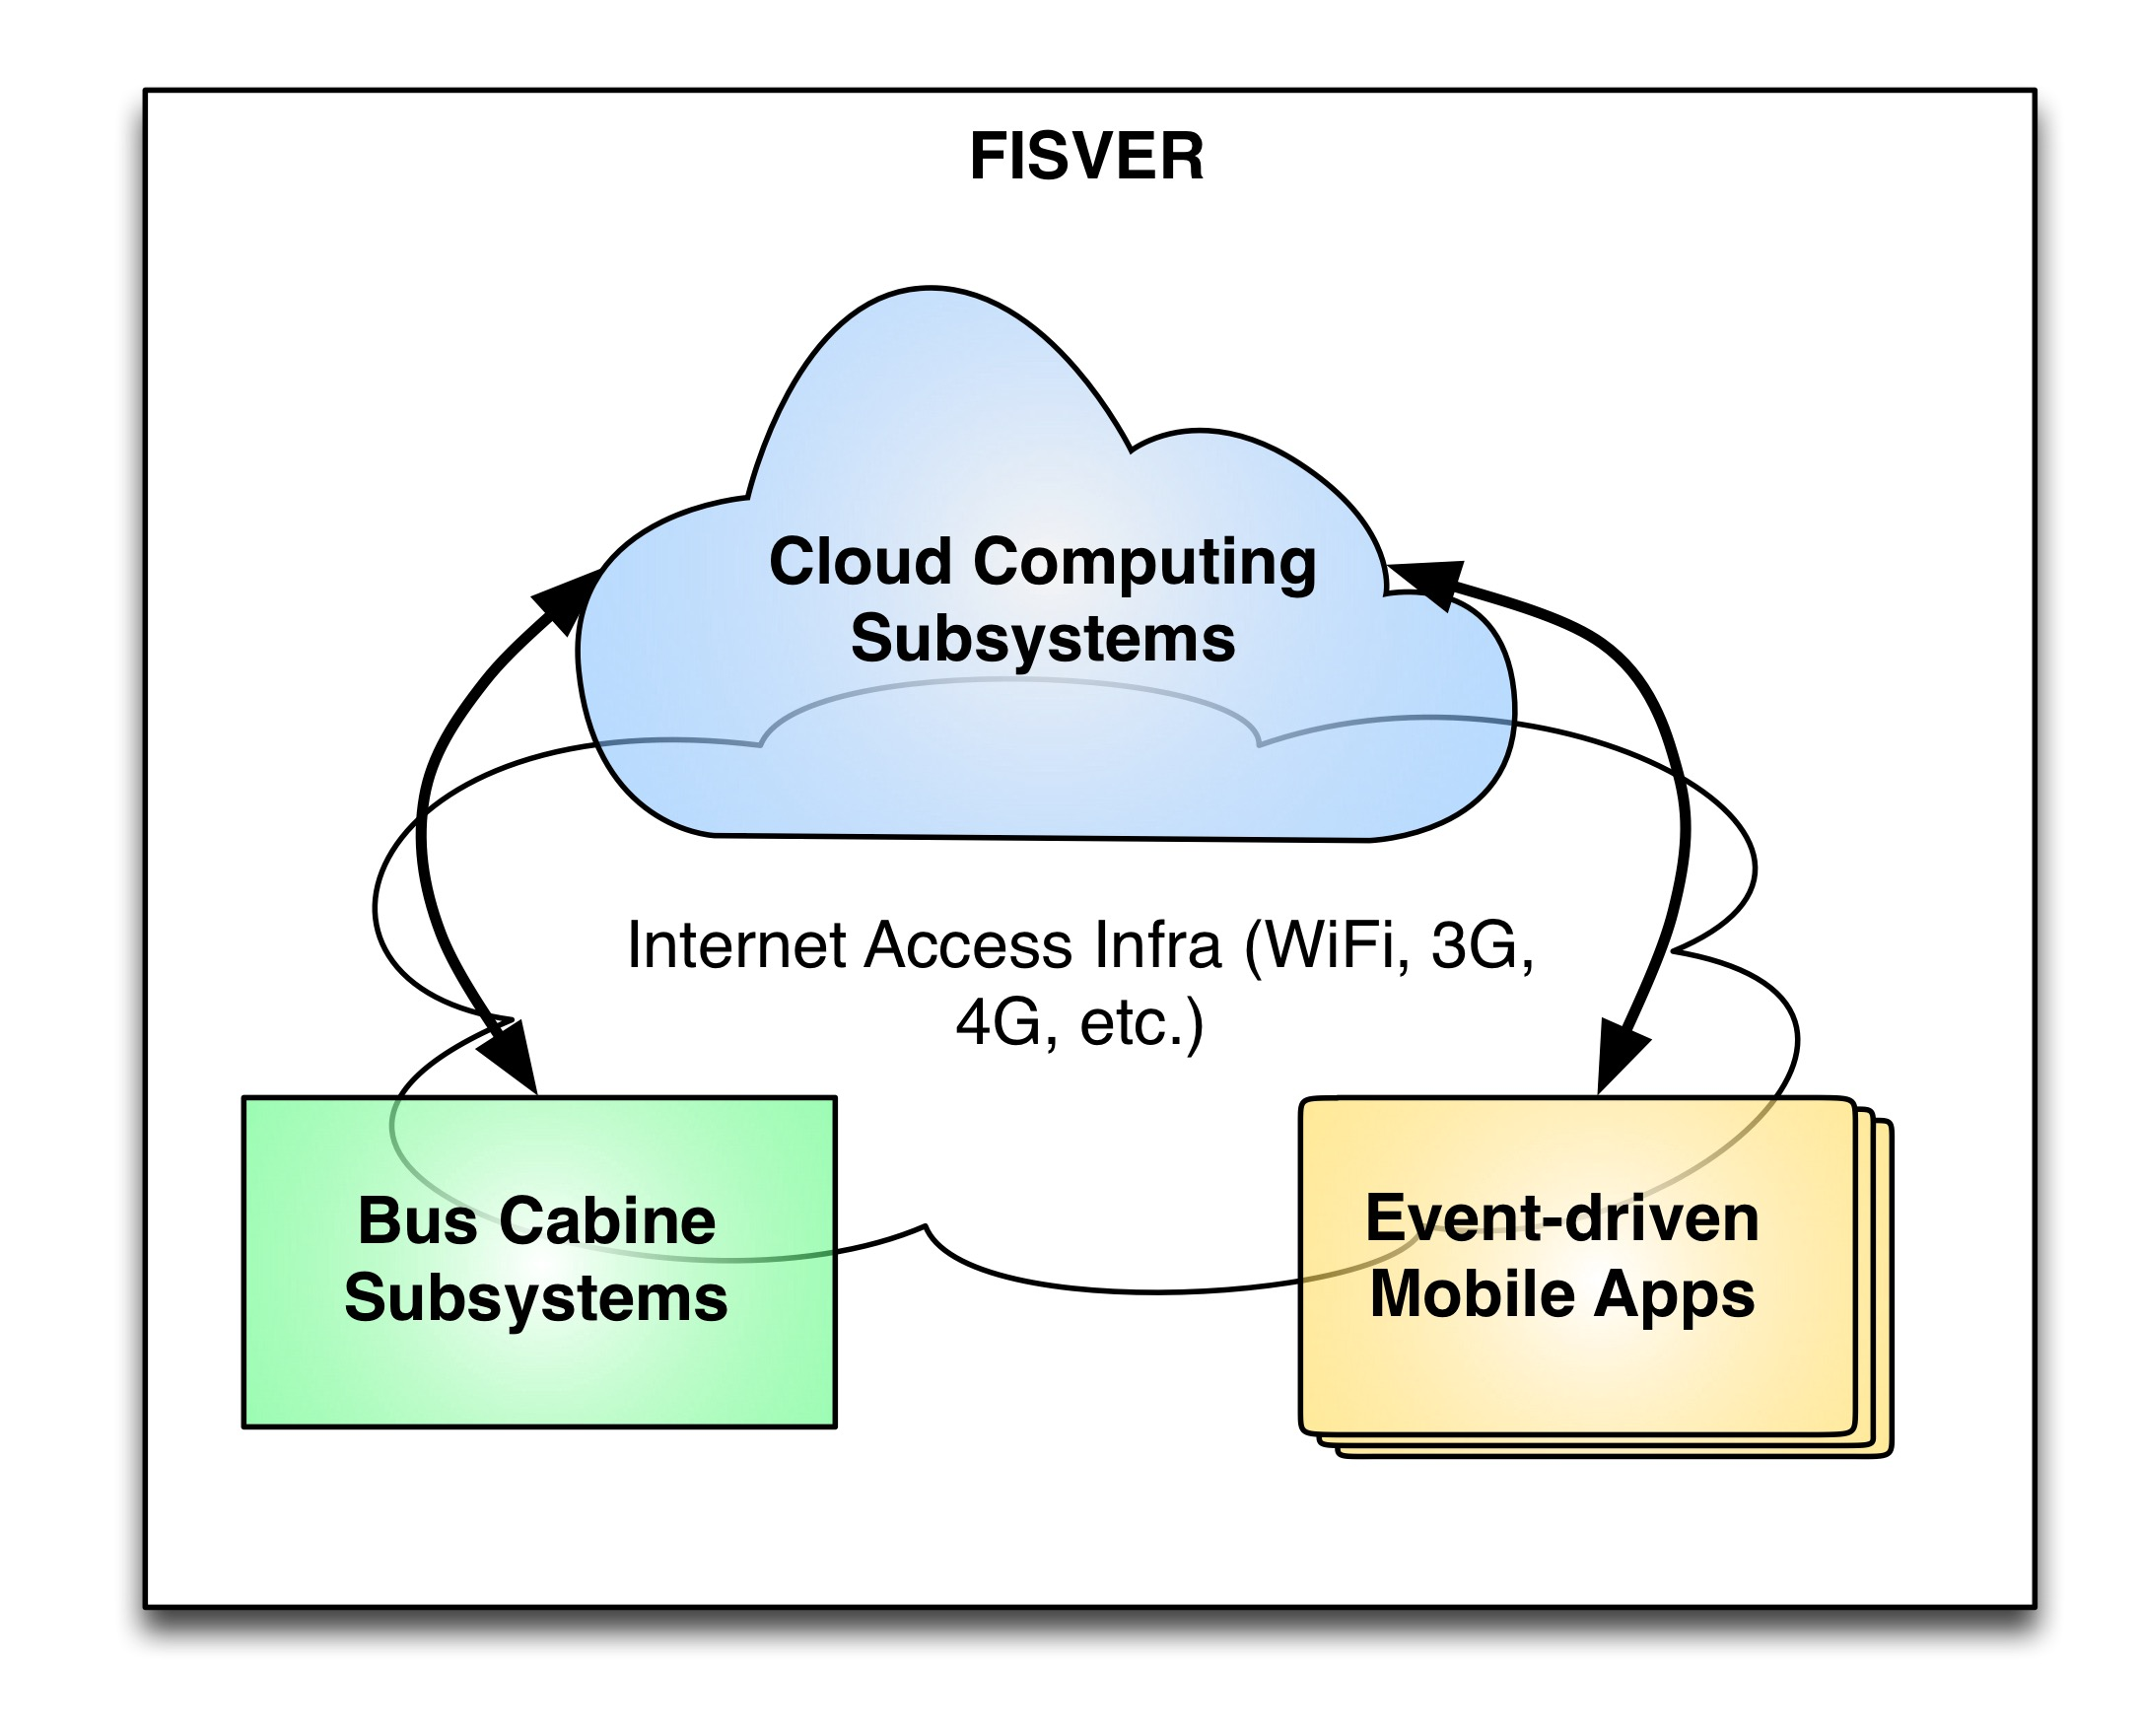
\includegraphics[scale=0.20]{Imagens/cap4_arch.png}
 	\caption{Main architecture for the proposed framework.}
 	\label{fig:arch}
\end{figure}

The FISVER key architecture is designed following a modular approach that features three interworking subsystems accessible via well-defined web-based external interfaces. In the FISVER modular architecture, each subsystem has clear divisions between subcomponents, which can be replaced/updated without affecting the rest of the system (in contrast to the integrated architecture). Each subsystem has their own architecture, featuring subcomponents that communicate each other via well-known internal interfaces. The key FISVER subsystems are described below:

\begin{itemize}

\item Bus Cabin Subsystems: This subsystem features a set of in-vehicle components responsible for: \textit{(i)} gathering sensory data in the bus cabin surrounding; \textit{(ii)} processing multimedia sensory data to afford identifying objects of potential security threats; \textit{(iii)} creating even crime level metadata; and \textit{(iv)} triggering the cloud infrastructure to provide crime level metadata for the targeted subsystems;

\item Cloud Infrastructure Subsystems: embeds a set of FISVER subsystems that exploit the powerful and scalable cloud computing infrastructure capabilities to afford large-scale storage, smart processing of sensory data and search of best suited crime assist units. The cloud services that can provisioned by the FISVER Cloud Infrastructure Subsystems are in the following: \textit{(i)} Templates as a Service, seeking to keep in-vehicle algorithms always up to date with new crime object patterns and/or new specific targets; \textit{(ii)} Event Classification as a Service, that exploits smart computing algorithms for classifying events in real-time based on the analysis in the image sent by the bus cabin subsystem; and \textit{(iii)} Crime Assist triggering as a Service, which addresses to find the best suited crime assist unit and further sending crime notifications to them for assistance;

\item Event-driven Mobile Apps: Runs on end user devices (e.g., smartphones/Tablets at crime assist units, third party safety centers, police authority control centers, etc.) deploying lightweight procedures. The event-driven mobile app is catheterized by mostly keeping in standby behavior until receiving crime notifications from the cloud Infrastructure subsystems, that are in turn presented to the users for appropriate assistance.
\end{itemize}

The FISVER approach is designed following the premise to run most complex smart computing procedures at the Bus Cabin and Cloud Infrastructure Subsystems. The FISVER approach foresees to achieve low networking overhead when compared to typical smart surveillance subsystems, since crime events may occur at lower periods of time (afforded by classifications of the cloud mechanisms). Moreover, typical smart surveillance subsystems keep constantly streaming multimedia data for remote processing, and beyond costly approach, such approach cannot guarantee QoE for assisting accurate detections. Details on each subsystem featuring the FISVER architecture are provided in the next.

\section{Bus Cabin Subsystems}

The Bus Cabin features a set of subsystems that are in charge to collect, process, and analyze multimedia data to detect crime threats in real-time. The Bus Cabin Subsystem key architecture design is depicted in Figure \ref{fig:buscabarq}.

\begin{figure}[htb!]
 	\centering
 	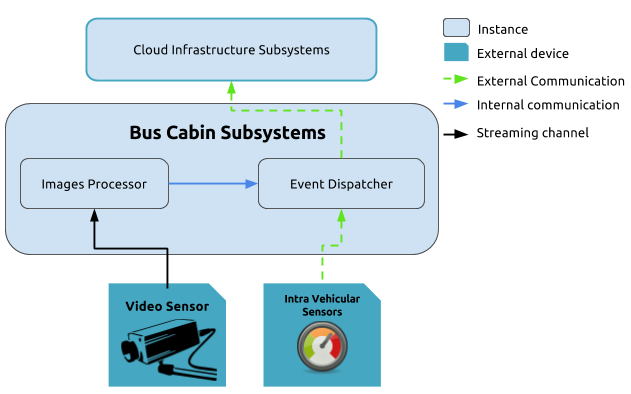
\includegraphics[scale=0.65]{Imagens/cap4_bus_cabin.png}
 	\caption{Bus Cabin Subsystem Architecture.}    
 	\label{fig:buscabarq}
\end{figure}
In next subsections \textbf{Images Processor} and \textbf{Event Dispatcher} are explained in details.
% * <augusto@dimap.ufrn.br> 2016-11-30T13:39:07.118Z:
%
% > FIGURA COM ARQUITETURA DO BUS-COMABIN MOSTRANDO Images Processor + Event Dispatcher + Intra-vehicular Sensors.
%
% Colocar figura da arquitetura do Bus Cabin aqui, e a seguir os subsistemas serão explicados. FAZER ISSO COM TOSO OS DEMAIS MODULOS QUE COMPÕE O FISVER........
%
% ^ <email@hugobarros.com.br> 2016-11-30T23:17:50.828Z:
%
% Feito
%
% ^.
\subsection{Images Processor}
% * <augusto@dimap.ufrn.br> 2016-11-30T13:19:33.415Z:
% 
% Ao que parece o modulo Bus Cabin é composto por Images Processor + Event Dispatcher+ mais algum? o tal Intra-vehicular Sensors? Vc deveria primeiramente apresentar a arquitetura geral do Bus Cabin Subsystem que mostre TODOS os subsistemas desse modulo e suas interfaces, e depois cada um deve ser descrito em suas devidas sub-sessões.
% 
% ^ <email@hugobarros.com.br> 2016-11-30T23:32:45.291Z:
%
% Feito acima, como descrito no comentário anterior. Os sensores são dispositivos externos.
%
% ^.
The Images Processor module is designed for downloading and updating the definitions in the algorithm configuration, for making new instances of image processing algorithms (one for each configuration), for comparing the input streaming in an attempt to find the specific target object, in which each algorithm was designed for, and lastly for storing definitions necessary for deploying algorithms. \ref{fig:buscab} depicts key features of the \textbf{Images Processor}.

\begin{figure}[htb!]
 	\centering
 	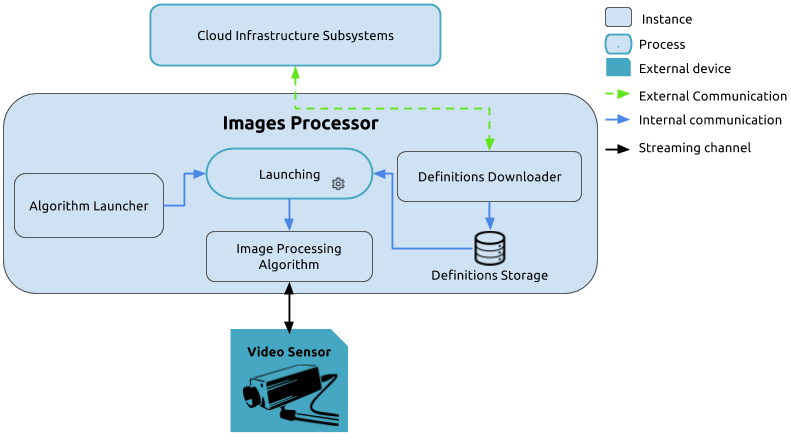
\includegraphics[scale=0.60]{Imagens/cap4_img_proc.png}
 	\caption{Features of Images Processor Subcomponent.}    
 	\label{fig:buscab}
\end{figure}

The key subcomponents featuring the Images Processor module are:
% * <augusto@dimap.ufrn.br> 2016-11-30T13:22:40.193Z:
% 
% > The key subcomponents featuring the Images Processor module are:
% > \begin{itemize}
% > \item \textbf{Definitions downloader:} at system bootstrap this component verifies if a new version or some new definition is available. In case of a new definition it will be downloaded and stored else if there is a new version of a definition it will be updated.
% > \item \textbf{Definitions Storage:} this component is responsible for storing all definitions and delivery them on query actions from algorithm instantiator.
% > \item \textbf{Algorithm instantiator:} after all definitions are downloaded and stored, the instantiator creates a new instance of each registered algorithm, passing as parameter the e specific configuration file containing parameters for one target object. All of them consuming the same streaming channel to collect and process images.
% ONDE ESTÁ O IMAGE PROCESSING ALGORITHM? ELE ESTÁ NA FIGURA APRESENTADO COMO UM SUBCOMPONENTE. E TEM AINDA O INSTATIATION (QUE PARECE NÃO SER UM SUBCOMPONENTE, MAS UMA ACÃO). SE FOR UMA AÇÃO NÃO DEVERIA CONSTAR NUMA FIGURA QUE APRESENTA UMA ARQUITETURA, POIS NÃO SE DESTINA A APRSENTAR AÇÕES, MAS COMPONENTES E INTERFACES. Ou não é uma figura de arquitetura mas um diagrama de fluxo?????? Defina isso e proceda como tal.
% 
% ^ <email@hugobarros.com.br> 2016-11-30T23:34:07.444Z:
%
% A figura é de fato da arquitetura, mas como a legenda mesmo mostra instantiation é um processo.
%
% ^.
\begin{itemize}

\item \textbf{Definitions downloader:} at system bootstrap this component verifies if a new version or some new definition is available. In case of a new definition it will be downloaded and stored else if there is a new version of a definition it will be updated.
\item \textbf{Definitions Storage:} this component is responsible for storing all definitions and delivery them on query actions from algorithm launcher.
\item \textbf{Algorithm launcher:} after all definitions are downloaded and stored, the launcher creates a new instance of each registered algorithm, passing as parameter the e specific configuration file containing parameters for one target object. All of them consuming the same streaming channel to collect and process images.
\end{itemize}
 
\textbf{Definitions Downloader} subcomponent, verifies if new version of definitions is available at \textbf{Cloud Infrastructure Subsystems}. It verifies too if a new object definition is registered. In this cases, definitions are downloaded and stored, for utilization at algorithms instantiation process. 
% * <augusto@dimap.ufrn.br> 2016-11-30T13:24:12.264Z:
%
% > invoked  at the system bootstrap
%
% A figura 4.2. apresenta que o Definitions Downloader é ativado no system bootstrapp???? NÃO, tem apenas módulos e setas.......aprenda rapaz.....
%
% ^ <email@hugobarros.com.br> 2016-11-30T23:35:16.713Z:
%
% corrigido
%
% ^.
Algorithm launcher in turn, creates an algorithm instance for monitoring images searching for a target object definition match. Images are acquired through a streaming channel, that are utilized by all algorithm instances. Details about Images Processor API subcomponents implementation with it methods and it parameters are shown in Table \ref{table algdep}.
% * <augusto@dimap.ufrn.br> 2016-11-07T22:34:17.937Z:
%
% > 1. ???
% > 2. ????
% > 3. ????
%
% Descrever em detalhes as funções disponíveis, a que se destinam cada uma, qual o resultado da implementação de cada, qual a sequência, etc etc etc.
%
% ^ <email@hugobarros.com.br> 2016-11-22T01:25:37.718Z:
% 
% feito em forma de tabela... faltando apenas uma forma de fazer merge nas celulas que possuem os nomes dos subcomponentes tornando a tabela mais organizada
% 
% ^.
\begin{center}
  \captionof{table}{Images Processor Subcomponent API}
  \label{table algdep} % for use in \ref{table1} if you want to refer to the table number
  \begin{tabular}{|c|c|c|c|c|c|}
  % etc.
  \end{tabular}
\end{center}
%\taburowcolors[2] 2{tableLineOne .. tableLineTwo}
%\tabulinesep = ^4mm_3mm
\tabulinesep=2.0mm
%\everyrow{\tabucline[.4mm  white]{}}

    \begin{tabu} to \textwidth {l >{\bfseries}X[r, 1.5] X[4,l,m]}
        \tableHeaderStyle
        
         & Method & Definition \\
       {\multirow{2}{*} {\rotatebox[origin=c]{90}{ \textbf{Defs. Downloader} }}} &verifyDef()&\small queries at cloud subcomponents if a new definition of of target object its available if yes download it and store it.\\
&verifyVers()&\small for each stored version of definitions this method verifies if a newer version is available, case true the local target object definition is updated.\\ \hline
\multirow{5}{*} {\rotatebox[origin=c]{90}{  \textbf{Definitions Storage} }}&\small getDefinition(String object)&\small returns latest version of a specific target object passed as parameter.\\
&\small getDefinition(String object, Integer version)&returns a passed as parameter version of a specific target object definition passed as parameter.\\
&\small addDefinition(String object)&\small creates a new version from a definition of target object passed as parameter. If no version exists for an object a new entry will be created for that object definition.\\
&\small purgeDefinition(String object)&\small Method utilized by \textbf{Definitions Downloader} in case of an old target object has been removed from system administrators .\\ \hline
{\rotatebox[origin=c]{90}{ \textbf{Algorithm Launcher} }}&init()&\small this method is called at finish of Definition Downloader tasks and is the last task of \textbf{Images Processor} bootstraping. It instantiates the image processing algorithms \\
\tabuphantomline
\end{tabu}
    
\hfill    
    
The sequence of interactions made between \textbf{Image Processor} subcomponents and their methods is shown in Figure \ref{fig:imgprocseq}. As described at the sequence diagram, \textbf{Definitions Downloader} triggers \textbf{Cloud Infrastructure} components following two main system events. 

\begin{figure}[htb!]
 	\centering
 	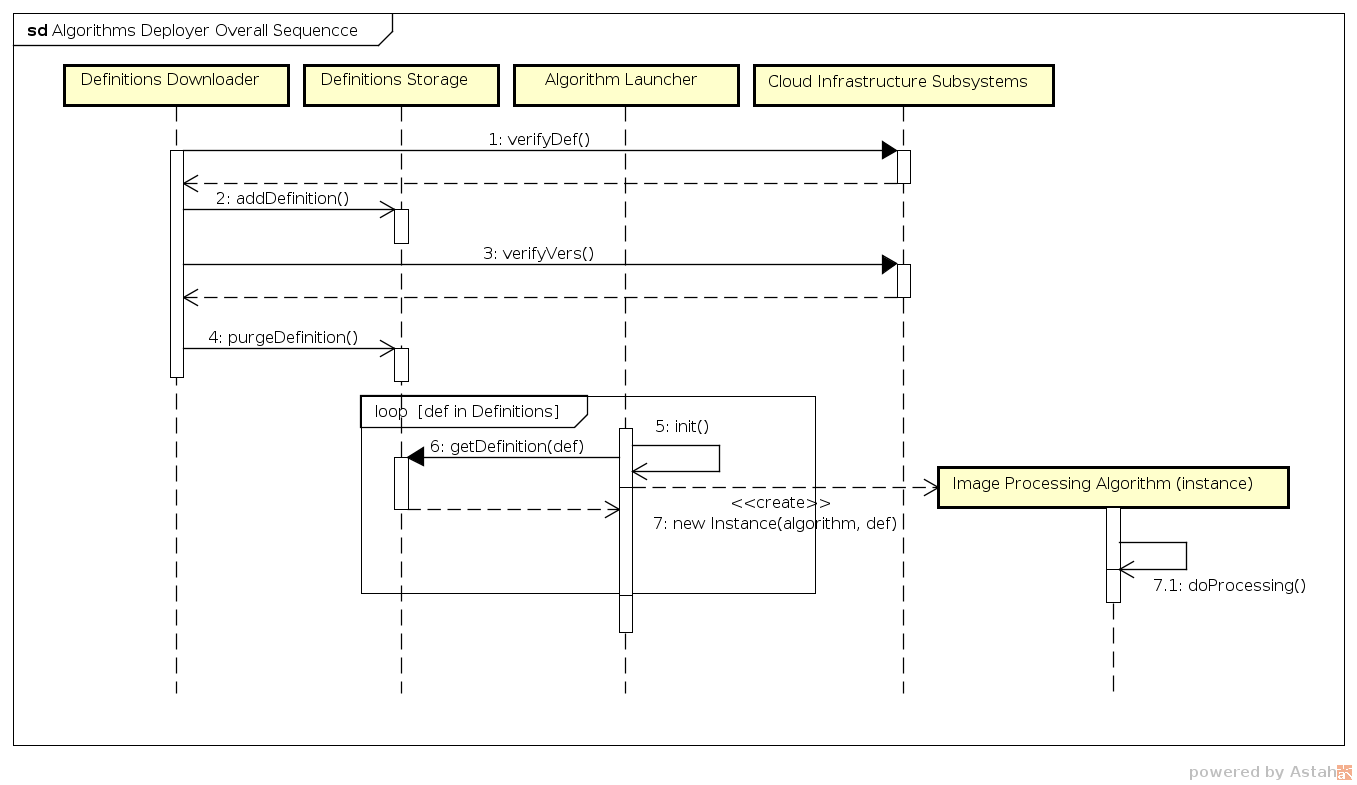
\includegraphics[scale=0.45]{Imagens/cap4_algseq.png}
 	\caption{Images Processor subcomponents overall sequence.}
 	\label{fig:imgprocseq}
\end{figure}

First for definitions updates, where existing objects definitions must be renewed. And second, for new target object definition registering, this occurs when new objects are registered at training phase, when system administrator collects several images of a target object for definitions extractions. 

% * <augusto@dimap.ufrn.br> 2016-11-23T18:21:57.279Z:
%
% > The sequence of interactions made between subcomponents and their methods described above is show in the sequence diagram below:
%
% Que sequencia? Descrito acima onde???? Não faça isso, use o nome da operação ou procedimento correspondente a sequência de interações que vc se refere.....não complica
%
% ^ <email@hugobarros.com.br> 2016-11-30T23:37:18.295Z:
%
% me referi ao diagrama de sequencia fig:imgprocseq
%
% ^.



% * <augusto@dimap.ufrn.br> 2016-11-30T12:25:30.013Z:
%
% > Instantiator
%
% Essa palavra "Instantiator" não existe no dicionário Inglês.......difícil viu
%
% ^ <email@hugobarros.com.br> 2016-11-30T23:58:09.935Z:
%
% Corrigido -> Algorithm launcher
%
% ^.

%\begin{figure}[htb]
% 	\centering
% 	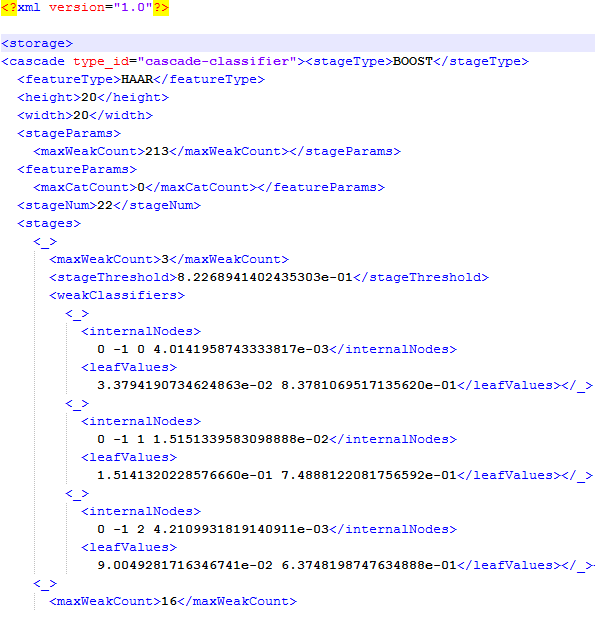
\includegraphics[scale=0.75]{Imagens/cap4_xml.png}
% 	\caption{Example of a configuration of an XML file.}
% 	\label{fig:xml}
%\end{figure}
% * <augusto@dimap.ufrn.br> 2016-11-07T22:30:03.855Z:
%
% > \begin{figure}[htb]
% >  	\centering
% >  	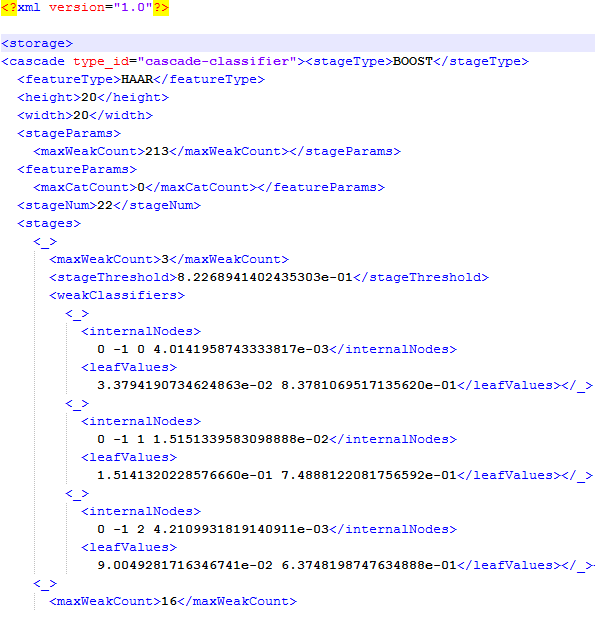
\includegraphics[scale=0.75]{Imagens/cap4_xml.png}
% >  	\caption{Example of a configuration of an XML file.}
% >  	\label{fig:xml}
% > \end{figure}
%
% Perceba que essa figura não aparece no item a que ela se destina apresentar, Bus Cabin Subsystem no caso, mas no texto ela vem no item de Cloud. Tem de haver uma maneira de controlar o posicionamento das figuras, porque simplesmente no texto INTEIRO isso ocorre, e só dá problema de entendimento e organização. 
%
% ^ <email@hugobarros.com.br> 2016-11-18T20:33:32.934Z:
%
% Resolvido... transformado em listing
%
% ^ <augusto@dimap.ufrn.br> 2016-11-30T12:23:32.085Z.


\subsection{Event Dispatcher Subcomponent}

The \textbf{Event Dispatcher} module is designed to aggregate information from both the \textbf{Images Processor} and the intra vehicular sensors(external devices). Once an event has been detected, this information is grouped in another XML type file which is prepared and sent to the for \textbf{Cloud Infrastructure Subsystems}. 
% * <augusto@dimap.ufrn.br> 2016-11-30T12:26:18.615Z:
% 
% "Images Processor and the Intra Vehicular Sensors"
% Cara, onde estão definidos esses subsistemas???? NENHUMA FIGURA das arquiteturas dos subsistemas constam estas entidades......Cara, tu não tem nenhum cuidado com isso, mostra tua total irresponsabilidade e desleixo com o trabalho.
% 
% ^ <email@hugobarros.com.br> 2016-11-30T23:59:17.488Z:
%
% external devices... corrigido
%
% ^.

\begin{figure}[htb!]
 	\centering
 	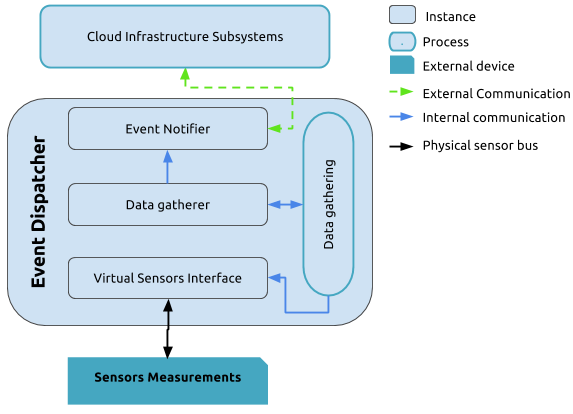
\includegraphics[scale=0.70]{Imagens/cap4_evtdspt.png}
 	\caption{Features of Event Dispatcher Subcomponent.}    
 	\label{fig:evtdspt}
\end{figure}

The subcomponent supported at the Event Dispatcher are:

\begin{enumerate}

\item \textbf{Event Notifier:} this subcomponent is responsible for collect data extracted from array of sensors an send it to \textbf{Cloud Infrastructure Subsystems}. As example: GPS location of bus at event moment, vehicle speed and fire sensor, but there are no limit for data extracted from any sensor available and registered for sensing.
\item \textbf{Data gatherer:} makes an edge from \textbf{Event Notifier} and sensors. The data is collected from sensor through a interface which implements an abstract layer for real sensor information. In this component data can be normalized, and converted when necessary.
\item \textbf{Virtual Sensors Interface:} this interface implements a virtual layer for data sensing. The sensor data can be collect from different sources each one with an specific protocol. So this interface realizes sensor data collection between different protocols.

\end{enumerate}

As said previously, \textbf{Event Dispatcher} component is called when an \textit{algorithm instance} matches a given image with a target object configuration. When this occurs, \textbf{Event Notifier} is called by an \textit{algorithm instance} and through \textbf{Virtual Sensors Interface} it collects all available sensory data to compose event message(aggregated in a XML file as exemplified in Listing \ref{event_file}).

\textbf{Data Gatherer} subcomponent is utilized at this step, for provide raw sensor data conversions(when necessary). For each registered sensor it can, do it based on the sensor interface implementation. It also verifies when sensor data is availabe or not for data collecting. 

For many causes, a sensor become unavailable and the process of collecting this sensor data may cause some delays. In this case \textbf{Data Gatherer} make array of sensors availability control for avoiding this kind of issue.

The \textbf{Event Notifier} that works at top of \textbf{Event Dispatcher} stack. It receive an \textit{algorithm instance} call, and after all process done by the \textbf{Data Gatherer} it prepares an event XML file, that will be sent to \textbf{Cloud Infrastructure Subsystems} in which receives this events through a web service.


In Listing \ref{event_file}, is shown an example of a generated XML file to report an event occurrence by the \textbf{Event Notifier}:

\begin{changemargin}{0.5cm}{0.5cm} 
\begin{center}
\begin{lstlisting}[caption={Example of an event XML file.},label={event_file},language=XML]
<?xml version="1.0"?>
<event>
    <!-- Potential threat event instance --!>
  <bus id="9999">
    <location>
      <lat>5.840592</lat>
      <long>-35.1999164</long>
    <location>
    <company id="45">
      <name>Example Company</name>
      <line>45</line>
  </bus>
  <avg_speed>40</avg_speed>
  <fire>false</fire>
  <algorithm  id="1001" name="cascade_classifier">
    <image_res>640_480</image_res>
    <detectime></detectime>
  </algorithm>
  <image_cut>
    R0lGODlhPQBEAPeoAJosM//AwO/AwHVYZ/z595kzAP/s7P+goOXMv8+
  </image_cut>  
</event>  
\end{lstlisting}
\end{center}
\end{changemargin}

In making it possible to establish communication with the \textbf{Cloud Infrastructure Subsystems} web service, the \textbf{Event Dispatcher} was designed to send grouped information (sensors, detectors and classifiers) in one compressed XML file(as in example shown above). Sensor Measurements, are external sensing devices, which are acessed through a textit{class} that implements \textbf{Virtual Sensors Interface}. This data is collected through an ODB2\footnote[19]{ODB2 connection implemented by \textbf{Virtual Sensors Interface}. http://www.obdii.com/. \textit{Accessed on December 10th, 2015.}} bus that can acquire data about the factory sensors e.g. speed, engine details, temperature etc.

In table \ref{table evt} a detailed description is shown for each method in \textbf{Event Dispatcher} subcomponent:

\begin{center}
  \captionof{table}{Event Dispatcher API}
  \label{table evt} % for use in \ref{table1} if you want to refer to the table number
  \begin{tabular}{|c|c|c|c|c|c|}
  % etc.
  \end{tabular}
\end{center}
%\taburowcolors[2] 2{tableLineOne .. tableLineTwo}
%\tabulinesep = ^4mm_3mm
\tabulinesep=2.0mm
%\everyrow{\tabucline[.4mm  white]{}}

    \begin{tabu} to \textwidth {>{\bfseries}l >{\bfseries}X[r, 1.5] X[4,l,m]}
        \tableHeaderStyle
        
         & Method & Definition \\
        {\multirow{2}{*} {\rotatebox[origin=c]{90}{Event Notifier}}}&\small prepareEvent(AlgEvent algevt)&\small receives an object with all details related to \textbf{Images Processor} processing. With this signaling, \textbf{Event Dispatcher} will make operations necessary to aggregate all data to report an event.\\
&sendEventNotification()&\small prepares, export and send a package within XML file format to \textbf{Cloud Infrastructure Subsystems}, this package contains all information about an event.\\ \hline
{\multirow{2}{*} {\rotatebox[origin=c]{90}{Data gatherer}}}&\small isAvailable(Integer sensorID)&\small verifies if a sensor is turned on and at normally functioning. Returns \textit{true} in positive case and \textit{false} in other cases.\\
&getAvailableData()&\small query all available sensor information normalizing and converting them when necessary.\\ \hline
{\multirow{2}{*} {\rotatebox[origin=c]{90}{Virtual Sensor Interface}}}&\small registerSensor(Integer sensorID, Class <class>)&\small creates a virtual sensor with an id. The implementation of real data the will be extracted from this sensor are made by a java class passed as parameter.\\
&getData(Integer sensorID)&\small instantiates the class registered for the specific sensor passed as parameter, and realizes all operations implemented for real data recovery.\\
\end{tabu}

\hfill

\textbf{Event Notifier} receives a call from \textbf{Images Processor}, which pass as parameter an object containing details about the target object matching, including image crop of acquired image containing the matched object. 
\textbf{Data Gatherer} in turn is called, which will look for all available sensors. Once available sensors are enumerated, all available data is collected using \textit{getAvailableData()} method. In this step a conversions and data treatment can be done depending on type of sensor and desired data.

\begin{figure}[htb!]
 	\centering
 	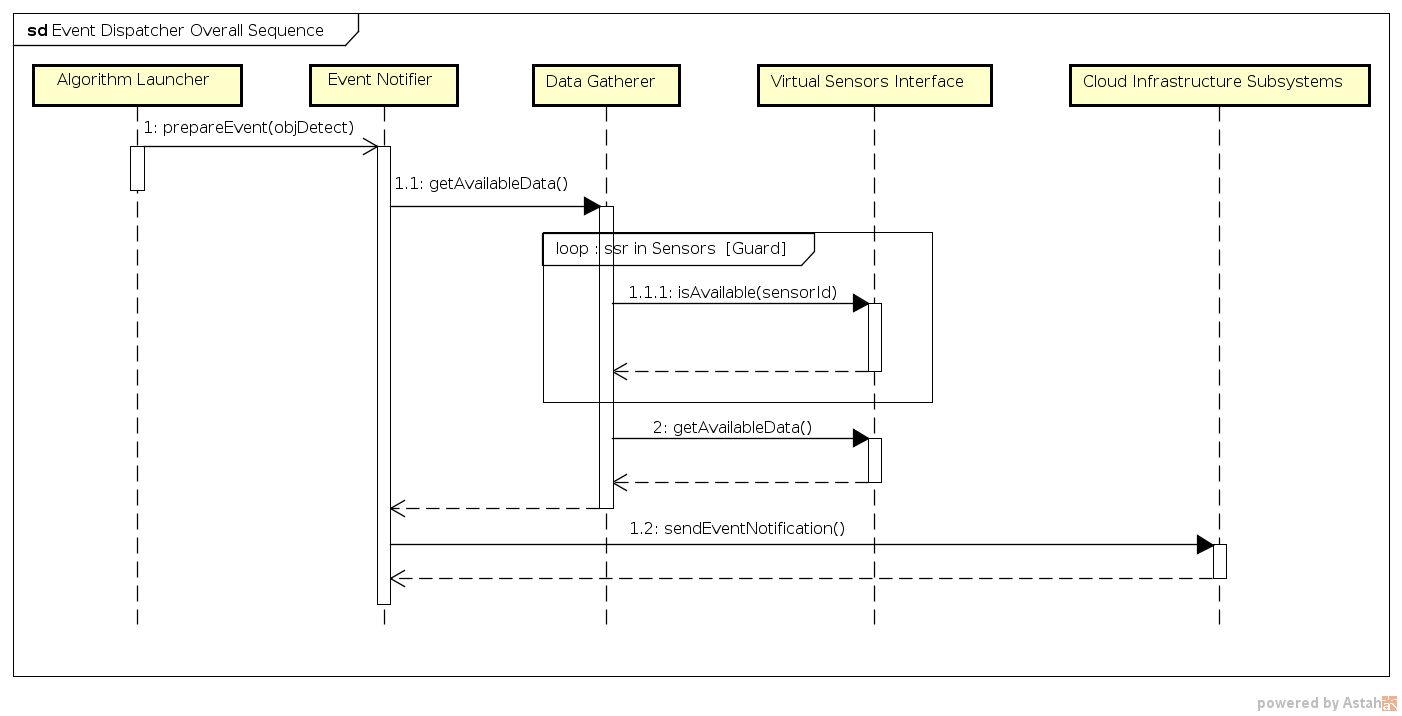
\includegraphics[scale=0.45]{Imagens/cap4_evtdsp.png}
 	\caption{Event Dispatcher subcomponent overall sequence.}
 	\label{fig:evtseq}
\end{figure}

\textbf{Virtual Sensors Interface} serves raw sensor data information to \textbf{Data Gatherer} subcomponent. It has functions for registering sensor and collect sensor raw data. In registering phase, done through \textit{registerSensor()} method, a \textit{class} that implements all details of raw data acquirement is passed as parameter. This classes implements \textbf{Virtual Sensor Interface} and are also responsible to implement details for sensors measurements acquirement, as example ODB2 communication for factory vehicle sensors measurements. The access of this sensors data can be made through serial port or Bluetooth \footnote[20]{Bluetooth Technology. https://www.bluetooth.com/. \textit{Accessed on December 10th, 2015.}} and this \textit{class} will be responsible for treating this assessment. After all this steps, \textbf{Event Notifier} send full event information to \textbf{Cloud Infrastructure Subsystems} through the method \textit{sendEventNotification()}. This communication is done through web service, and the information received will be treated by subcomponents that will be described at next subsection.


\section{Cloud Infrastructure Subsystems}

The Cloud Infrastructure Subsystem are in charge for deploying smart procedures to classify the received crime threats indications, and if confirmed, best suited crime assist unit(s) is(are) then searched and triggered to deal with the crime at the location. The FISVER approach relies on the possibility to benefit the overall system with the large-scale performance capabilities (i.e., processing, storage, and other key resources) that are commonly provisioned by the cloud-capable infrastructures. In Figure \ref{fig:cloud_infra}, there is a description of key component designs that will be deployed in a specific cloud provider to support both the Bus Cabin components and Event-driven Mobile Application.

\begin{figure}[htb!]
 	\centering
 	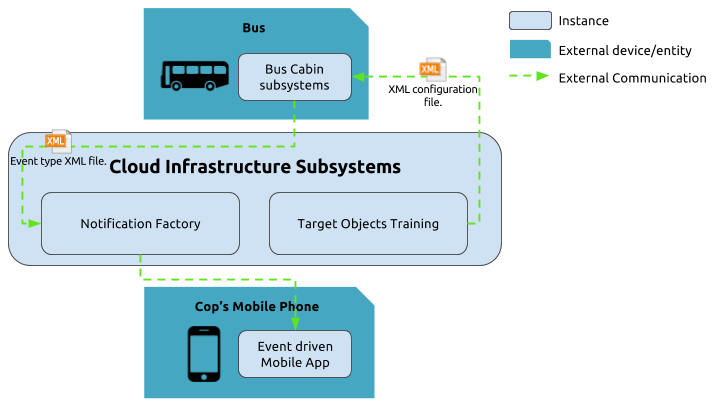
\includegraphics[scale=0.65]{Imagens/cap4_cloud_infra.png}
 	\caption{Cloud Infrastructure Subsystems Architecture.}
 	\label{fig:cloud_infra}
\end{figure}

The intercommunication between the Bus Cabin and the Cloud Infrastructure subsystems is carried out through SOAP\footnote[21]{SOAP W3C Specification. https://www.w3.org/TR/soap/. \textit{Accessed on December 10th, 2015.}} Web Service specification. Layers interaction are illustrated in the Figure \ref{fig:soap} below:

\begin{figure}[htb!]
  \centering
  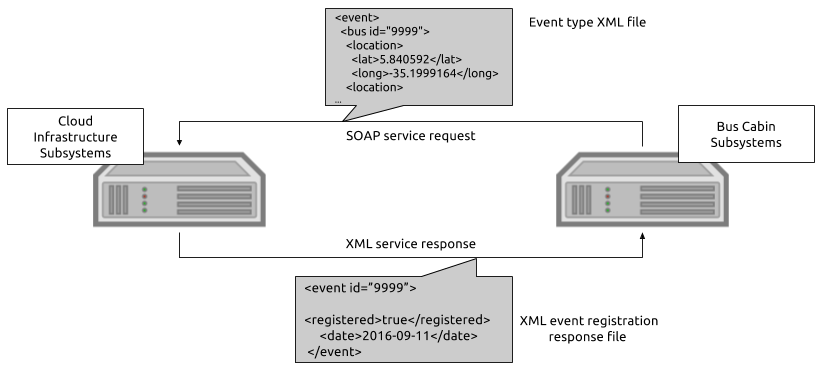
\includegraphics[scale=0.50]{Imagens/cap4_soap_arq.png}
  \caption{SOAP communication overview between FISVER layers.}
  \label{fig:soap}
\end{figure}

Figure \ref{fig:soap}, shows an example of message swapping between \textbf{Bus Cabin Subsystems} and \textbf{Cloud Infrastructure Subsystems} at the moment of a crime threat detection. In this example an Event notification is sent as a SOAP service request. As response \textbf{Bus Cabin Subsystems} receives information related to event registration (as example \textit{id} and \textit{date}). At next subsections, details about \textbf{Target Object Training} and \textbf{Notification Factory} subcomponents are given.

%https://www.w3.org/2000/xp/Group/
% * <augusto@dimap.ufrn.br> 2016-11-07T22:39:21.758Z:
%
% > The intercommunication between the Bus Cabin and the Cloud Infrastructure subsystems is carried out through...
%
% webservice???? Como se comunicam? Nao basta dizer que um manda mensagem ao outro, COMO ISSO É FEITO? Que protocolo? Quais mensagens são definidas na Accebility interface???? Que funções estão disponíveis????? Po, tu não uma planilha no excel pra isso, são aplicações que funcionam em rede.......
%
% ^ <email@hugobarros.com.br> 2016-12-01T04:55:48.664Z:
%
% in progress
%
% ^.

\subsection{Target Object Training}
% * <augusto@dimap.ufrn.br> 2016-11-07T22:50:47.924Z:
%
% > Target Object Training}
%
% Descreva em subitens todos os subcomponentes de cada subsistema, com todas as informações necessárias e as devidas especificações e elementos que possam descrever isso
%
% ^ <email@hugobarros.com.br> 2016-12-01T04:56:10.680Z:
%
% feito na versão anterior
%
% ^.
\begin{figure}[htb!]
  \centering
  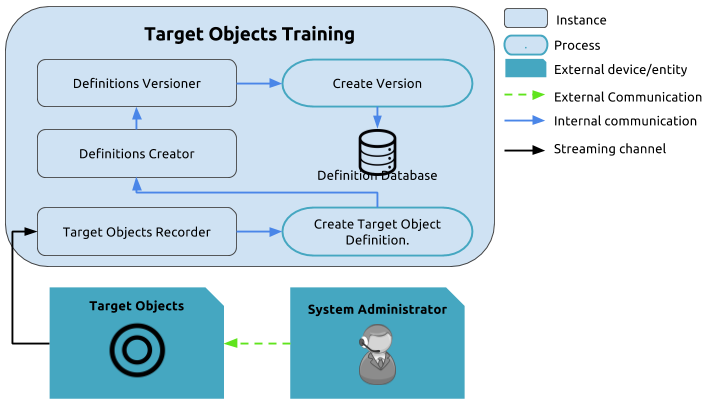
\includegraphics[scale=0.65]{Imagens/cap4_objtraining.png}
  \caption{Object Training Subcomponent.}
  \label{fig:objt}
\end{figure}
Since there is a wide range of target objects, the Target Object Training Module makes it possible to add new objects for purposes of recognition. These can only be accessed by the police authorities (i.e. a security analyst), who can insert, update or delete target object \textit{definitions}. The main task of \textbf{Target Object Training} is create, update and store target object \textit{ definitions} for updating all the \textbf{Bus Cabin} instances in which \textbf{Images Processor} subcomponent uses them through \textbf{Algorithm Launcher} as parameter for a target object matching. In Figure \ref{fig:objt} details about \textbf{Target Objects Training} subcomponent are depicted. The proposed approach creates \textit{definitions} for target object management. These definitions are based on the color and shape of the target objects. Data extracted from \textbf{Definitions Creator} subcomponent, creates a file containing relevant information such as the color of the gradient and shape of the objects. Definition extraction process is done through OpenCV\footnote[22]{Open Source Computer Vision Library. 
http://docs.opencv.org/2.4/index.html \textit{Accessed on December 10th, 2015.}} library. \textbf{Target Objects} are dangerous objects utilized in crime threats. They are selected by the system administrator before training phase for any causes. One cause is to improve \textbf{Bus Cabin} dispatched events(avoid false alarms) another cause is to add new set of \textbf{Target Objects} for \textbf{Images Processor} subcomponent matching(at \textbf{Bus Cabin Subsystems}).
For definitions creation is necessary a set of samples. There are two types of samples: negative and positive. Negative samples correspond to non-object images. Positive samples correspond to images with detected objects. Set of negative samples must be prepared manually, whereas set of positive samples is created using OpenCV API. \textbf{Target Objects Recorder} subcomponent is reponsible for acquire positives images(through a streaming channel) and store them temporally. \textbf{Definitions Creator} gets union of positives samples and generates \textit{definitions} based of features extracted from positives samples. The Listing \ref{config_file} shows an example of a \textit{definition} file created at this step: 
%Base64\footnote[18]{Online Decode. http://www.onlinedecode.com/about-base64/. \textit{Accessed on December 10th, 2015.}} image datasets for training when necessary. 

\begin{changemargin}{1.5cm}{1.5cm} 
\begin{center}
\begin{lstlisting}[caption={Example of a target object definition file.},label={config_file},language=XML]
<?xml. version="1.0"?> 
<!-- configuration file for a target object detection --!>
<storage> 
 <cascade type_id="cascade-classifier">
  <stageType>BOOST</stageType> 
   <featureType>HAAR</featureType> 
    <height>20</height> 
    <width>20</width> 
   <stageParams> <maxWeakCount>213</maxWeakCount> </stageParams> 
   <featureParams>  <maxCatCount>0</maxCatCount> </featureParams> 
   <stageNum>22</stageNum> 
   <stages> 
    <maxWeakCount>3</maxWeakCount> 
	<stageThreshold>8.2268941402435303e-01</stageihreshold>
	<weakClassifiers> 
	 <internalNodes> O -1 0 4.0141958743333817e-03</internalNodes>
	 <leafValues> 3.3794190734624863e-02 8.3781069517135620e-01
     </leafValues>
    </weakClassifiers>
    </stages>
</storage> 
\end{lstlisting}
\end{center}
\end{changemargin}

This XML file is generated during the training phase with extraction of features by positives target objects images. This features will be utilized by the \textbf{Algorithm Launcher} as a parameter in algorithm launching process at \textbf{Bus Cabin Subsystems}. Table \ref{table to} show detailed description about each \textbf{Target Objects Training} subcomponent methods:
\begin{center}
  \captionof{table}{Target Objects Training API}
  \label{table to} % for use in \ref{table1} if you want to refer to the table number
  \begin{tabular}{|c|c|c|c|c|c|}
  % etc.
  \end{tabular}
\end{center}
%\taburowcolors[2] 2{tableLineOne .. tableLineTwo}
%\tabulinesep = ^4mm_3mm
\tabulinesep=2.0mm
%\everyrow{\tabucline[.4mm  white]{}}

    \begin{tabu} to \textwidth {>{\bfseries}l >{\bfseries}X[r, 1.5] X[4,l,m]}
        \tableHeaderStyle
%% forma de fazer com multirow http://tex.stackexchange.com/questions/111249/multirows-multicolums-and-vertical-centring-in-the-tabu-environment        
         & Method & Definition  \\
        {\multirow{2}{*} {\rotatebox[origin=c]{90}{\small Target Objects Recorder}}}&trainNewObJ(Image[] imgarray)&{receives an image array from the new object to be recorded and extract it caracteristics, that will used for create definition.}\\
        &trainExistingObj(Image[] imgarray, boolean merge)&{update an object definition, based on new image array passed as parameter, with option to merge current definition with new or overwrite all definitions with new images, signaled by boolean parameter merge.}\\ \hline
{\multirow{2}{*} {\rotatebox[origin=c]{90}{Defs. Creator}}}&consolidateTraining()&{realizes validation in definitions created by \textbf{Target Object Definition processs} and generates XML definition file that will be passed for \textbf{Definitions Versioner}}.\\
&mergeDefinitions(Integer defIDFrom, Integer defIDTo)&{merges passed as id parameter the definitions, this method is called by \textbf{Target Objects Recorder} when the update process of an existing object was called passing the merge parameter with \textit{true} value.}\\ \hline
\rotatebox[origin=c]{90}{Defs. Versioner}&defineVersion(Integer objectID, Definition def)&{based on a registered object this method defines how different a previous version is from the newer that will be addded to \textbf{Definitions Database}, gived a new version number, this objects will be stored at \textbf{Defs Database}.}\\ \hline
{\multirow{2}{*} {\rotatebox[origin=c]{90}{Definitions Database}}}&storeDef(Integer objectID, Definition def, Version ver)&{ stores a passed as parameter definition, related to an object passed as parameter too.}\\
&getCurrentDefs()&{ returns all active \textit{Target Ojbects Definitions}. This  method is used by the all instances of \textbf{Images Processor} in it bootstraping to make objects updates.}\\

\end{tabu}
\hfill

When \textit{definition} creation process is completed, \textbf{Definitions Versioner} is called to verify if already exists a trained target object definition, if doesn't exists, a new entry is created for that objects as primary version. Case already exists, definition will receive a new version that will be registered for that target object and stored at \textbf{Definitions Database}. 
At the finish of \textit{definition} creation, a file containing target objects feature extraction values is generated. This values will be used by all \textbf{Bus Cabin Subsystems} instances when updated through \textbf{Definitions Downloader} subcomponent as detailed in previous section. After checking any changes in the \textbf{Definitions Database} the \textbf{Definitions Versioner} module generates a new target object definition version. The \textbf{Definitions Database} handles the storage of all the textit{definition} versions and their creation of data, as well as noting the users who created them and their observations.

% * <augusto@dimap.ufrn.br> 2016-08-22T21:56:12.822Z:
%
% Essa figura precisa ser explicada passo a passo, comentando a sequência realizada no diagrama. Eu acho que a especificação neste capítulo é mt insuficiente, parece descrever uma coisa muito simples (6 páginas). Use e abuse de diagramas, como diagramas de estado, isso enriquece o capítulo principal da dissertação, que descreve a proposta em "detalhes"....mas carede dos tais detalhes.
%
% ^ <augusto@dimap.ufrn.br> 2016-10-16T23:59:27.499Z:
%
% Isso aqui não foi feito no documento, o que falta? Explica o diagrama de sequência....
%
% ^.

% * <email@hugobarros.com.br> 2016-10-05T19:55:20.110Z:
%
% https://www.websequencediagrams.com/
%
% ^ <email@hugobarros.com.br> 2016-11-05T21:30:22.494Z.


%The \textit{Data Gathering} module acts as an interface between the Bus Cabin and Cloud Components, and checks each new Alert package to find out if the quality of the information meets the requirements necessary before the security analysts can be notified . If the \textit{Data Gathering} approves the quality of the %\textit{contextualAlertPackage}, it is sent to the \textit{Publish Manager} who is called on to publish the alert to the mobile applications.

\subsection{Notification Factory}

\textbf{Notification Factory} subcomponent, is responsible for receive \textit{event notifications}, sent by all \textbf{Bus Cabin Subsystems} instances. In Figure \ref{fig:notfact} details about \textbf{Notification Factory} subcomponent architecture are shown:

%The Data Gathering module receives all the information sensed by the bus cabin system; and this information can be further made use of by deploying the applications in the proposed cloud services. The purpose of the Publish Manager is to catalog communication information and send it to an interested context-driven application whenever an event occurs. 

%In Figure \ref{fig:workflow}, there is a generic workflow which explains more clearly the updated templates, object detection, context generation and publishing process.
%At least one object template registered at Templates Database is required to initiate the recognition procedure. Once the Templates Database is populated, the Object Detector can retrieve templates and start the detection process. If the similarity measure reaches a threshold (which is established by security analysts as a parameter), the Object Detector will notify the Event Manager about the region that is matched with a target object template. Event Manager, in turn collects the sensor information (GPS, Velocity, etc.) and creates a contextual Alert Package by sending it to Data Gatherer. 

%\begin{figure}[htb!]
% 	\centering
% 	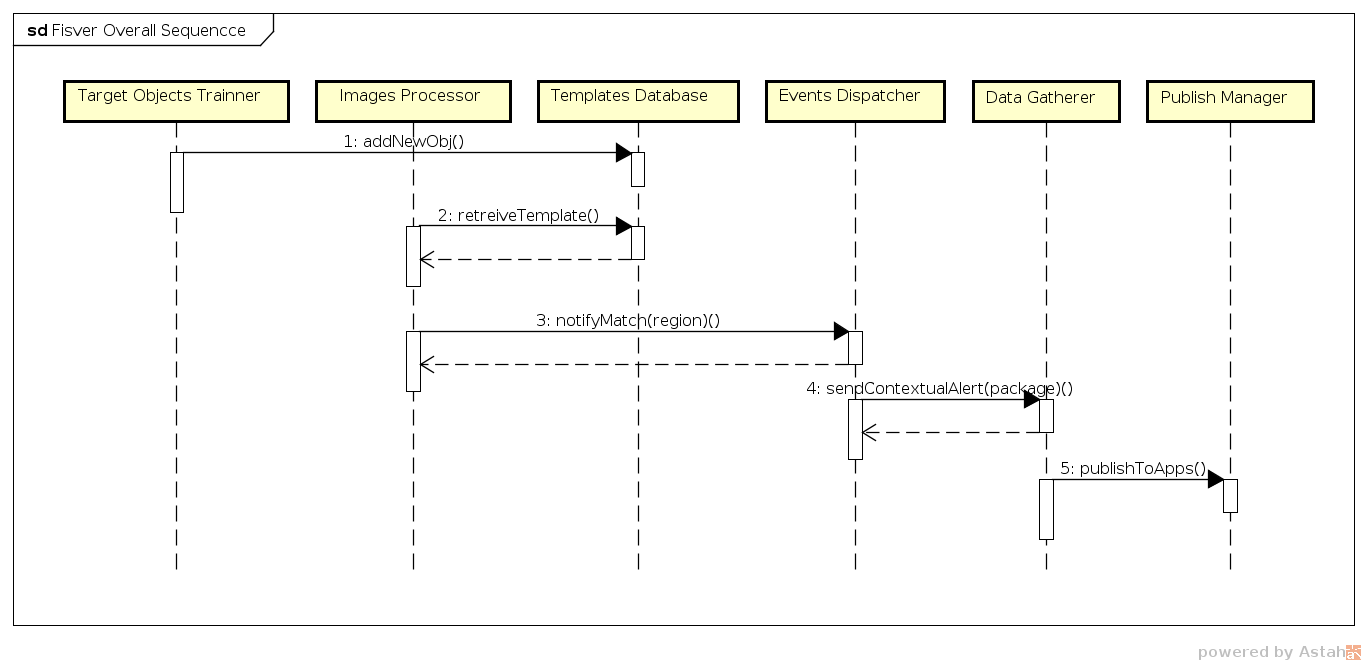
\includegraphics[scale=0.45]{Imagens/cap4_fisver_over_seq.png}
% 	\caption{Fisver cloud components overall sequence.}
% 	\label{fig:workflow}
%\end{figure}



%At least one object template registered at \textit{Templates Database} is required to initiate the recognition procedure. Once the \textit{Templates Database} is populated, the \textit{Object Detector} %can retrieve templates and start the detection process. If the similarity measure reaches a threshold (which is established by security analysts as a parameter), the \textit{Object Detector} will notify %the \textit{Event Manager} about the region that is matched with a target object template. \textit{Event Manager}, in turn collects the sensor information (GPS, Velocity, etc.) and creates an Alert %Package by sending it to \textit{Data Gathering}. 

\begin{figure}[htb]
 	\centering
 	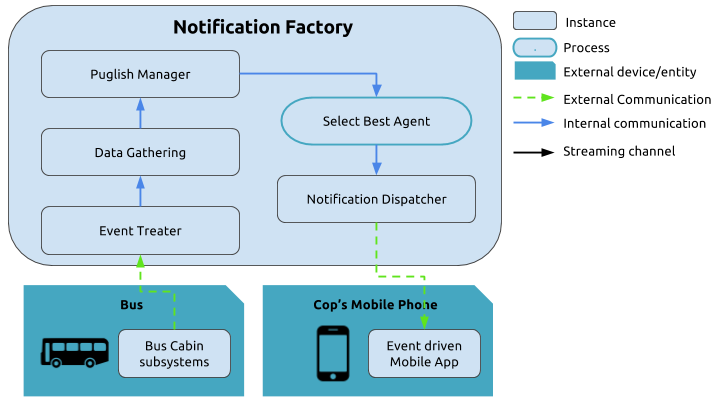
\includegraphics[scale=0.65]{Imagens/cap4_notffact.png}
 	\caption{Notification Factory Subcomponent.}
 	\label{fig:notfact}
\end{figure}
Once a threat \textit{event} is dipatched from \textbf{Bus Cabin Subsystems}, the \textbf{Event Treater} subcomponent is able to make validations about that received event. In order guarantee \textbf{Cloud Subsystems} service continuity, \textbf{Event Treater} works with a processing queue in which, incoming \textit{events} are received and queued for a validation process in order to discard wrong \textit{events} messages. This validation is made over \textbf{Bus Cabin Subsystem} entry if it has a valid registered \textit{id}. In \textit{event} validation process, \textit{sensors measurements} are also validated to avoid triggering all \textbf{FiSVER} stack to alert about a wrongly sent event, as example an \textit{event} in which sensed \textit{GPS location} reports an event at a jungle, where is impossible to ride by bus.
In table \ref{table notf}, we show each method specification:

\begin{center}
  \captionof{table}{Notification Factory API}
  \label{table notf} % for use in \ref{table1} if you want to refer to the table number
  \begin{tabular}{|c|c|c|c|c|c|}
  % etc.
  \end{tabular}
\end{center}
\tabulinesep=2.0mm
    \begin{tabu} to \textwidth {>{\bfseries}l >{\bfseries}X[r, 1.5] X[4,l,m]}
        \tableHeaderStyle
        
         & Method & Definition  \\
    	Event Treater&receiveEvent()&receives an \textit{event notification} and realizes all validations necessary to forward event to next subcomponents.\\
        Data Gathering&unpackEvent()&makes received event unpacking and register event details for analysis. \\
Publish Manager& publishNotification() &Selects the best(nearest) agent to deliver the notification.\\
Notification Dispatcher&sendNotification()&Prepares notification and send it to selected agent.\\

\end{tabu}



The \textit{unpackEvent()} method, calls all \textit{Classes} with \textbf{Data Gathering} interface implementation. The \textbf{FISVER} approach, turns possible addition of new actions at \textbf{Cloud Infrastructure} layer. This actions are implemented by classes with \textbf{Data Gathering} abstract methods implementations, containing all details for registering events and making decisions, as event delivering or not.

%\begin{figure}[htb!]
% 	\centering
% 	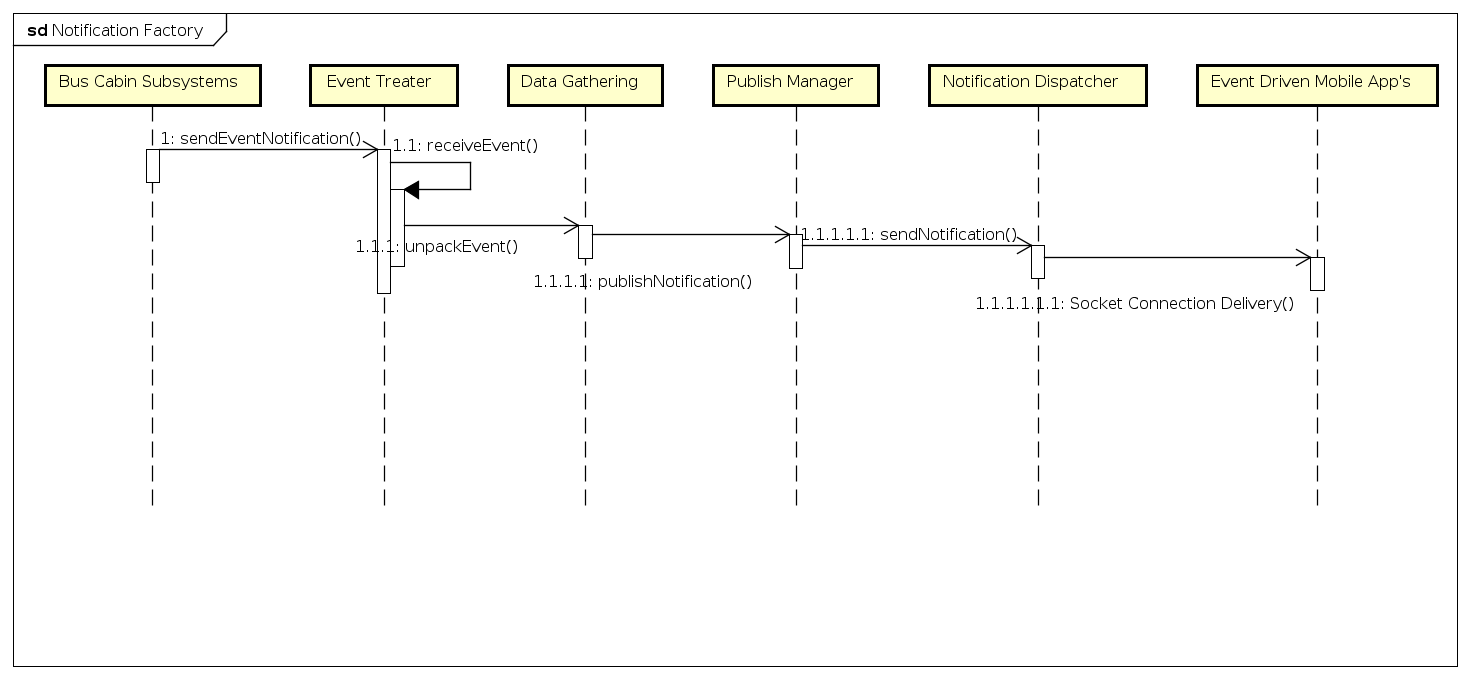
\includegraphics[scale=0.45]{Imagens/cap4_notifackseq.png}
% 	\caption{Notification Factory operation sequence.}
% 	\label{fig:seqnotfac}
%\end{figure}



\section{Event-driven Mobile Applications}
% * <augusto@dimap.ufrn.br> 2016-11-07T22:52:09.386Z:
%
% > Event-driven Mobile Applications}
%
% Especifique a aplicação, diagrama de estado dela, como é ativada (webservice????), que metadados ela recebe, benefícios do event-driven, ETC ETC ETC ETC. Vc acha que e parágrafos minúsculos e esta figura descrevem isso?
%
% ^.
Currently, proven cloud services can facilitate the development of any application, whether it be mobile or desktop. In view of the benefits expected from the components set out in the proposed framework cloud model, a wide range of applications for smart public safety can be anticipated. In light of this, we designed an Event-driven mobile application use case as a \textit{"proof-of-concept"} as an easy way to integrate and deploy applications through the use of FISVER. In Figure \ref{fig:app} an event alert was sent to a police agent smartphone:


\begin{figure}[htb]
 	\centering
 	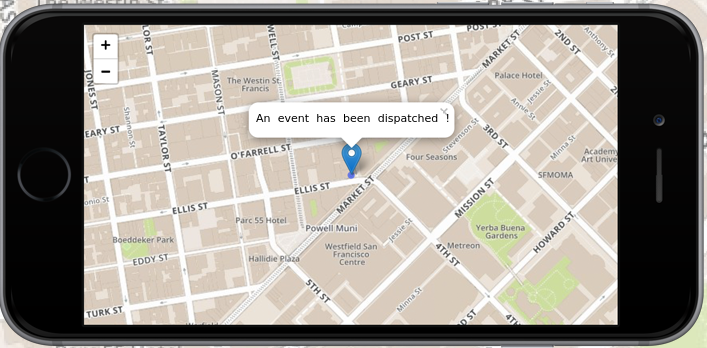
\includegraphics[scale=0.50]{Imagens/cap4_app.png}
 	\caption{Prototype of a Mobile application.}
 	\label{fig:app}
\end{figure}


The information extracted from several instances and grouped in the proposed framework can benefit governments by offering them new opportunities to plan and maintain a lot of applications. One example of an application considered in this scenario was employed in the police car, probably in a tablet or in the cop's smartphone that contains the GPS location. 

With the aid of this information the nearest police car can be warned by receiving an alert about a crime event occurring in a bus, together with the bus directions (future location of the bus in a street or venue) and thus make any intervention easier.
% * <augusto@dimap.ufrn.br> 2016-08-22T21:59:21.740Z:
%
% Acho que vc poderia fechar este capítulo com a descrição de um Use Case,  para concretamente exemplificar o uso da ferramenta, e tbm somar mais ao capítulo que está mt pobre enquanto especificação....
%
% ^.
\section{Conclusion}
% * <augusto@dimap.ufrn.br> 2016-08-22T21:57:57.608Z:
%
% Overview?????? Não né, o capítulo dis "Detailed descriptio.....", e não overview. Vc precisa descrever em detalhes, muitos detalhes.......não reflete isso este caoítulo....
%
% ^.
In this chapter, there was an overview of the FISVER architecture. Details about each \textbf{FISVER} \textit{subcomponent} were described as well as the interaction all of them. The next chapter will include an evaluation of the scenarios and results.